\part{MIMO预编码}
\section{点对点MIMO系统}
\subsection{系统模型}
\begin{equation}
    y=Hx+z
\end{equation}
其中,$y\in C^{N_r\times1}$,$x\in C^{N_t\times 1}$,$z\in C^{N_r\times1}$,发送端总能量为$E\{x^Hx\}=P$,噪声功率谱密度为$N_0$,即$E\{zz^H\}=N_0I_{N_r}$,且
\begin{equation}
    \begin{aligned}
        R_{yy}&=E\{yy^H\} \\
        &=HR_{xx}H^H+N_0I_{N_r}
    \end{aligned}
\end{equation}

\subsection{系统容量}
\begin{equation}
    \begin{aligned}
        I(x;y)&=H(x)-H(x|y)\\
        &=H(y)-H(y|x) \\
        &=H(y)-H(Hx+z|x) \\
        &=H(y)-H(z|x) \\·
        &=H(y)-H(z)
    \end{aligned}
\end{equation}
其中,$z$是满足复高斯随机分布的多维向量,因此当且仅当$y$也满足复高斯随机分布时,上式取得最大值,且
\begin{equation}
\begin{aligned}
    H(y)&=log_2|\pi eR_{yy}| =log_2|\pi eHR_{xx}H^H+\pi eN_0I_{N_r}| \\
    H(z)&=log_2|\pi e N_0I_{N_r}|
\end{aligned}
\end{equation}
于是,
\begin{equation}
    I(x;y)=log_2\left|I_{N_r} + \frac{HR{xx}H^H}{N_0}\right|
\end{equation}

\subsection{传输侧无CSI}
假设每根天线上的发送信号能量相等且相互独立,即$R_{xx}=\frac{P}{N_t}I_{N_t}$,则
\begin{equation}
    \begin{aligned}
    C&=log_2\left|I_{N_r} + \frac{P}{N_tN_0}HH^H\right| \\
    &=\sum_{i=1}^{N_t}log_2(1+\frac{P}{N_tN_0}\lambda_i)
    \end{aligned}
\end{equation}

\subsection{传输侧有CSI}
预编码提高信道容量 \\
对信道矩阵$H$使用SVD分解,即$H=U\Sigma V^H$,一般假设$Nr>Nt$,则
\begin{equation}
\Sigma=\left[ 
    \begin{matrix}
        \sqrt{\lambda_1} & 0 & \cdots & 0 \\
        0 & \sqrt{\lambda_2} & \cdots & 0 \\
        \vdots & \vdots & \ddots & \vdots \\
        0 & 0 & \cdots & \sqrt{\lambda_{N_t}} \\
        \vdots & \vdots & \vdots & \vdots \\
        0 & 0 & 0 & 0
    \end{matrix}
\right] 
\end{equation}
令调制后信号能量表示为$\tilde{x}$,预编码后的发送信号能量为$x=V^H\tilde{x}$,则

\begin{equation}
    \begin{aligned}
    y &= Hx+z \\
    &=U\Sigma V^HV\tilde{x}+z \\ 
    &=U\Sigma\tilde{x}+z
    \end{aligned}
\end{equation}  
\begin{equation}
    U^Hy = U^HU\Sigma\tilde{x}+U^Hz =>
    \tilde{y}=\Sigma\tilde{x}+\tilde{z}
\end{equation} 


上式展开为
\begin{equation}
\left[
    \begin{matrix}
        \tilde{y}_1 \\
        \tilde{y}_2 \\
        \vdots \\
        \tilde{y}_{N_t} \\
        \vdots \\
        \tilde{y}_{N_r}
    \end{matrix}
\right]
=\left[ 
\begin{matrix}
    \sqrt{\lambda_1} & 0 & \cdots & 0 \\
    0 & \sqrt{\lambda_2} & \cdots & 0 \\
    \vdots & \vdots & \ddots & \vdots \\
    0 & 0 & \cdots & \sqrt{\lambda_{N_t}} \\
    \vdots & \vdots & \vdots & \vdots \\
    0 & 0 & 0 & 0
\end{matrix}
\right]
\left[
\begin{matrix}
    \tilde{x}_1 \\
    \tilde{x}_2 \\
    \vdots \\
    \tilde{x}_{N_t}
    \end{matrix}
    \right] + 
    \left[
\begin{matrix}
    \tilde{z}_1 \\
    \tilde{z}_2 \\
    \vdots \\
    \tilde{z}_{N_t} \\
    \vdots \\
    \tilde{z}_{N_r}
\end{matrix}
\right]
\end{equation}

即
\begin{equation}
    \tilde{y}_i=\sqrt{\lambda_i}\tilde{x}_i+\tilde{z}_i, i=1,\cdots,r.一般\ r=N_t
\end{equation}
原始的MIMO信道等效为$r$个SISO信道,每个SISO信道的信道容量可以表示为:
\begin{equation}
    C_i(P_i)=log_2(1+\frac{\lambda_iP_i}{N_0})
\end{equation}
其中,$P_i$表示第$i$根天线上的信号能量,且
\begin{equation}
    E\{x^Hx\}=\sum_{i=1}^{N_t}E\{|x_i|^2\}=\sum_{i=1}^{N_t}P_i=P
\end{equation}
于是,信道总容量为:
\begin{equation}
    C=\sum_{i=1}^{N_t}C_i(P_i)=\sum_{i=1}^{N_t}log_2(1+\frac{\lambda_iP_i}{N_0})
\end{equation}
可以通过注水算法优化功率分配,达到更大的信道容量,即
\begin{equation}
    \begin{aligned}
        & C={\underset{\{P_i\}} {\operatorname {arg\,max}}}\ \sum_{i=1}^{N_t}C_i(P_i)=\sum_{i=1}^{N_t}log_2(1+\frac{\lambda_iP_i}{N_0}) \\
        & s.t\ \  \sum_{i=1}^{N_t}P_i=P 
    \end{aligned}
\end{equation}
最优解为   
\begin{equation}
    \begin{aligned}
        P_i^{opt}&=(\mu -\frac{N_0}{\lambda_i})^+, i=1,\cdots,r \\
        \sum_{i=1}^{N_t}P_i&=P
    \end{aligned}
\end{equation}

\subsection{MIMO注水算法}
\begin{algorithm}
    \caption{注水算法}
    Step1:迭代计算p=1,计算$\mu=\frac{N_t}{r-\rho+1}$ \\
    Step2:用$\mu$计算$\gamma_i=\mu-\frac{N_tN_0}{E_x\lambda_i},i=1,2,\cdots,r-p+1$ \\
    Step3:若分配到最小增益的信道能量为负值,即设$\gamma_{r-p+1}=0,p=p+1$,转至Step1 \\
    若任意$\gamma_i$非负,即得到最佳注水功率分配策略
\end{algorithm}

\subsection{经典预编码算法}
参考文献\cite{2017Massive}
\paragraph{起源}
MIMO无线通信技术最早广泛应用于WiFi技术上(IEEE 802.11ac/n),WiMax技术(IEEE 802.16e),4G(LTE/LTE-A)等系统。最早的MIMO思想来源于点对点的MIMO系统,接着发展出了MU-MIMO,每个用户配备一个单天线。
\subsubsection{线性预编码}
\paragraph{Matched Filter(MF)}
\begin{equation}
    W_{MF} = \sqrt{\alpha} H^H
\end{equation}
\paragraph{ZF}
\begin{equation}
    W_{ZF} = \sqrt{\alpha} H(H^HH)^{-1}
\end{equation}
\paragraph{RZF(或MMSE)}
\begin{equation}
    W_{MMSE} = \sqrt{\alpha} H(H^HH+X+\lambda I_K)^{-1}
\end{equation}
\paragraph{TPE}
\begin{equation}
    W_{TPE} = \sum_{j=0}^{J-1}w_j(H^HH)^jH^H
\end{equation}
\paragraph{优缺点对比}
\par
优缺点如图\ref{kjdfgshafgdad}所示。
\begin{figure}[ht]
    \centering
    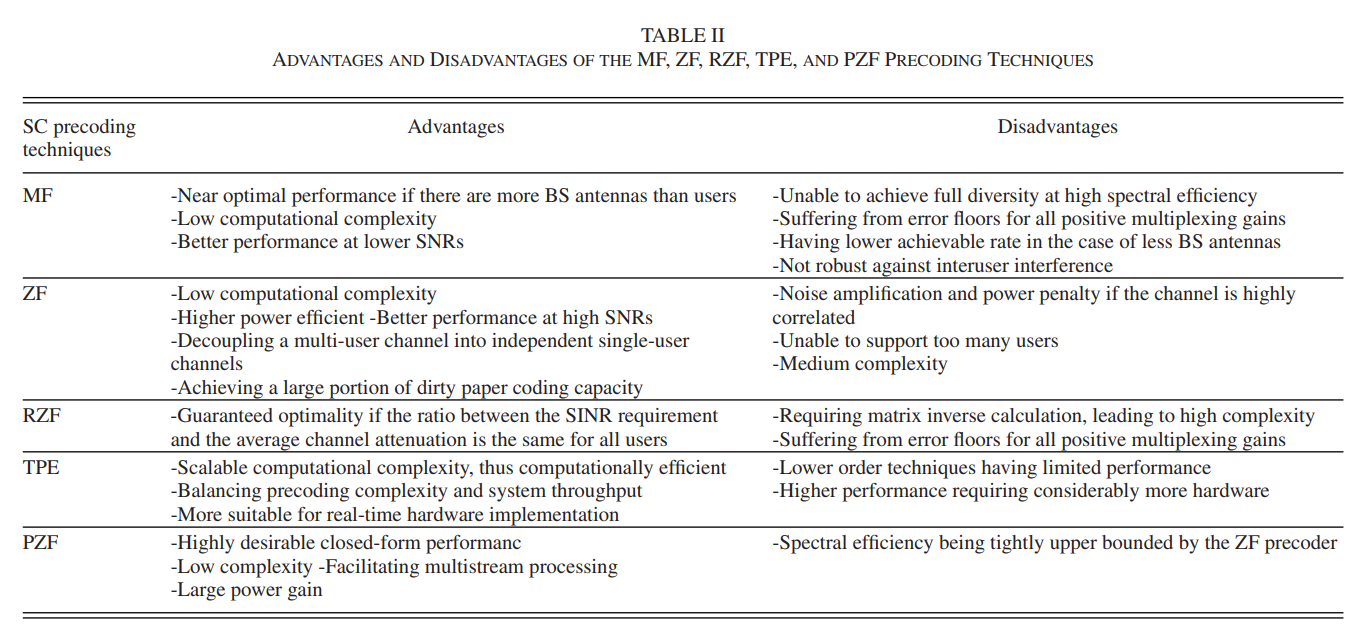
\includegraphics[width=0.99\textwidth]{线性precoder优缺点对比.PNG}
    \caption{优缺点对比}
    \label{kjdfgshafgdad}
\end{figure}

\subsection{基于AI的预编码算法}
\begin{enumerate}
    \item \emph{Kyeongbo Kong, Woo-Jin Song, Moonsik Min, Deep-learning-based precoding in multiuser MIMO downlink channels with limited feedback, 2008.0417}\par
        基于深度学习的均衡,反馈和预编码,下行MU-MIMO系统。基站侧发送预编码使用transmitter DNN实现,每个receiver DNN引入二值化层来模仿量化过程,从而使能端到端训练。由于二值化层的引入导致网络的梯度失真从而容易陷入局部极小值,网络训练过程中引入了辅助训练网络作为教导网络,有效避免陷入局部极小值。与传统的线性预编码相比,该网络通过端到端训练达到了更高的和速率。
    \item \emph{Novel MMSE Precoder and Decoder Designs Subject to Per-antenna Power Constraint
    for Uplink Multiuser MIMO Systems, I-Tai Lu, Jialing Li and Enoch Lu, 2009}\par
        关于多用户MIMO上行预编码的文章,理论比较多。文中提到,最经典的点对点MIMO系统在发送总功率一定时,最优预编码矩阵有最优解,但是在每根天线的功率有限或扩展到多用户MIMO,闭式解不存在,对于MU-MIMO,每个用户总功率有限时,可以通过两种方法寻找数值解,TCIO和GIA。
    \item \emph{Evolution of Uplink MIMO for LTE-Advanced}\par
        LTE中上行MIMO的技术介绍
    \item \emph{Deep Learning based Hybrid Precoding for mmWave Massive MIMO system using ComcepNet, 2020.7}\par
        提出了新的预编码网络结构”ComcepNet“,该网络结合了复数卷积块和 Inception 网络的特征,展现了比autoprecoder更好的性能。
    \item \emph{Deep Learning Based Precoder Design in MIMO Systems with Finite-Alphabet Inputs,2020}\par 
        有限元预编码
    \item \emph{Deep Learning for Distributed Channel Feedback and Multiuser Precoding in FDD Massive MIMO, 20.07}\par
        多用户信道估计和反馈问题可以视为一个分布式信源编码问题。与传统的每个用户独立估计信道信息不同,文章提出联合设计导频并且接收端使用DNN直接将接收导频映射为反馈bit,然后基站将所有用户的反馈bit直接映射为预编码矩阵,可以显著低提高整机性能。文章进一步提出鲁棒化设计策略,并且泛化DNN结构使之适应可变用户和可变的反馈bit。Numerical results show that the DNN-based approach with short pilot sequences and very limited feedback overhead can already approach the performance of conventional linear precoding schemes with full CSI.
    \item \emph{Deep Unfolding for Communications Systems: A Survey and Some New Directions,2019}\par 
        本文综述了深度展开的原理,并讨论了其在通信系统中的最新应用,重点讨论了多天线(MIMO)无线系统中的检测和预编码以及纠错码的信念传播译码。
    \item \emph{Deep reinforcement learning approach to MIMO precoding problem: Optimality and Robustness, 2020}\par 
        强化学习
    \item \emph{Model-Driven Deep Learning for Massive Multiuser MIMO Constant Envelope Precoding} \par 
        常包络预编码设计可以显著降低硬件损耗和功率损耗,但是已有的常包络预编码算法计算复杂度高。文章提出使用模型驱动的方式将深度学习与conjugate gradient algorithm结合,原始迭代算法展开并添加可训练参数,通过数据学习有效的参数。仿真结果表明该网络能有效抑制多用户干扰和计算复杂度。
    \item \emph{}
    
\end{enumerate}

\section{多用户MIMO下行系统}
\subsection{系统模型}
考虑一个由基站和$K$个相互独立的用户组成的单小区下行多用户MIMO系统,其中基站配置$M$根天线,用户$k$配置$N_k$根天线($k=1,2,\cdots,K$)。设基站向用户$k$发送的数据向量为$\bm{s}_k=[s_{k1},s_{k2},\cdots,s_{kN_k}]^T$,且每个用户的数据向量相互独立,发给每个用户的数据向量都经过一个预编码矩阵$\bm{V}_k\in \mathbb{C}^{M\times L_k}$,其中$L_k$为用户$k$所支持的数据流数目,满足$L_k\leq N_k$,则基站发送的信号为:
\begin{equation}
    \begin{aligned}
        \bm{x}&=\sum_{i=1}^K\bm{V}_i\bm{s}_i \\
        &=[\bm{V}_1,\bm{V}_2,\cdots,\bm{V}_K]\begin{bmatrix}
            \bm{s}_1 \\
            \bm{s}_2 \\
            \vdots \\
            \bm{s}_K            
        \end{bmatrix} \\
        &= \bm{V}\bm{s}
    \end{aligned}
\end{equation}
假设基站端发射功率限制为P,那么发送信号满足条件:
\begin{equation}
    \begin{aligned}
        \mathbb{E}\{tr(\bm{x}\bm{x}^H)\}&=\mathbb{E}\{tr(\bm{Vs}(\bm{Vs})^H)\} \\
        &=\mathbb{E}\{tr(\bm{V}\bm{V}^H)\} \\
        &=\sum_{i=1}^{K}tr(\bm{V}_i\bm{V}_i^H)\leq P
    \end{aligned}
    \label{dkjgdsjgjsdkh}
\end{equation}
用户$k$的接收信号可以表示为
\begin{equation}
    \begin{aligned}
    \bm{y}_k&=\bm{H}_k\bm{x} + \bm{n}_k \\
    &=\bm{H}_k\sum_{i=1}^{K}\bm{V}_i\bm{s}_i + \bm{n}_k \\
    \end{aligned}
    \label{jhagdjasgdj}
\end{equation}
其中,$\bm{H}_k\in \mathbb{C}^{N_k\times M}$为基站到用户的信道矩阵,$\bm{n}_k\sim \mathcal{CN}(\bm{0},\sigma^2 \bm{I}_{N_k}) $表示相应的加性独立同分布(i.i.d)高斯白噪声向量。将所有用户的接收信号统一表示为
\begin{equation}
    \bm{y}=\bm{H}\bm{x}+\bm{n}=\begin{bmatrix}
        \bm{H}_1 \\
        \bm{H}_2 \\
        \vdots \\
        \bm{H}_K 
    \end{bmatrix}
    \bm{x}+\bm{n}
\end{equation}\par 
式中,$\bm{H}=\begin{bmatrix}
    \bm{H}_1 \\
    \bm{H}_2 \\
    \vdots \\
    \bm{H}_K 
\end{bmatrix}=\begin{bmatrix}
    \bm{h}_{11} & \bm{h}_{12} & \cdots & \bm{h}_{1M} \\
    \bm{h}_{21} & \bm{h}_{22} & \cdots & \bm{h}_{2M} \\
    \vdots      & \vdots      & \ddots & \vdots      \\
    \bm{h}_{K1} & \bm{h}_{K2} & \cdots & \bm{h}{KM}
\end{bmatrix} \in \mathbb{C}^{\sum_{k=1}^{K}N_k\times M}$表示基站到用户的总信道矩阵,{\color{yellow}{其中元素$\bm{h}_{ij}$也是一个矩阵,表示第$j$根天线到第$i$个用户的信道矩阵}。}\par 
假设用户信道是平坦衰落的,基站端可以通过信道估计获得准确的信道状态信息,并且假设移动端知道自己的信道状态信息。下行链路CSI的获取:{\color{yellow}{TDD$\Longrightarrow$利用上下行信道互译性原理;FDD$\Longrightarrow$CSI反馈。}}\par 
将式$\ref{jhagdjasgdj}$写为如下形式:
\begin{equation}
    \begin{aligned}
        \bm{y}_k&=\bm{H}_k\sum_{i=1}^{K}\bm{V}_i\bm{s}_i+\bm{n}_k \\
        &=\bm{H}_k\bm{V}_k\bm{s}_k+\bm{H}_k\sum_{i=1,i\neq k}^{K}\bm{V}_i\bm{s}_i+\bm{n}_k
    \end{aligned}
    \label{sjkagdjhagdjhkasgf}
\end{equation}\par 
其中,\textbf{第一项表示期望接收信号,第二项表示共信道干扰(CCI)[也成为多用户干扰,MUI],第三项式噪声项},对于用户$k$来说第二项和第三项是毫无用处的,会影响用户信号的正常接收,因此线性预编码的主要目标就是{\color{yellow}{在一定的功率限制条件下,使得共信道干扰和噪声项的影响尽量小,最大化期望接收信号。}}
\subsection{MRT预编码}
由于可以平衡系统性能和计算复杂度,最大比传输(MRT)预编码【又称作匹配滤波器(MF)预编码】是最简单易实现的预编码算法,通过最大化接收信噪比(SNR)实现。在大规模MIMO系统中,当基站天线数$M$足够大时,最简单的MRT线性预编码方案便可以得到最优的系统性能。\par 
在发射端已知完美信道状态信息的前提下,MRT线性预编码矩阵为:
\begin{equation}
    \bm{V}=\beta_{MRT}\bm{H}^H
\end{equation} 
(注:以上编码矩阵后可以加上功率分配矩阵组成整个预编码矩阵)\par
式中,$\beta_{MRT}=\sqrt{\frac{1}{tr(\bm{H}\bm{H}^H)}}$为约束基站发送功率的约束因子。大规模MIMO系统中\textbf{基站天线数的不断增加使得信道矩阵列向量之间逐渐呈现正交性,即不同终端间的干扰逐渐降低甚至被完全消除},因此最简单的 MRT 预编码下便可以获得最优的频谱效率和最好的信号传输质量,且复杂度最低。\par 

传统MIMO系统中,匹配滤波预编码方案的侧重点在于接收端用户的信号增益最大化,但在多用户系统的场景下,随着传输信道相关性的提升,此方案由于没有考虑如何对用户间的干扰进行处理,将会导致整个系统性能快速下降。
\subsection{基于广义信道求逆的预编码}
\subsubsection{ZF预编码}
迫零预编码的主要思想是\textbf{利用信道的伪逆矩阵形式对发送数据进行编码处理,以达到完全消除其他用户干扰(共信道干扰)的目的}
由\ref{sjkagdjhagdjhkasgf}可知,为了消除CCI(即让第二项为0),预编码矩阵需满足:
\begin{equation}
    \bm{H}_k\bm{V}_i=\bm{0},i=1,2,\cdots,K,i\neq k
\end{equation}\par 
即,迫零预编码矩阵$\bm{V}_k$必须满足除目标用户$k$以外的其他用户联合信道矩阵$\tilde{\bm{H}_k}=\begin{bmatrix}
    \bm{H}_1 \\
    \vdots   \\
    \bm{H}_{k-1} \\
    \bm{H}_{k+1} \\
    \vdots       \\
    \bm{H}_K
\end{bmatrix}$的零空间内,信道矩阵的\textbf{伪逆}可以实现以上要求,$H$的伪逆矩阵为
\begin{equation}
    \bm{H}^+=\bm{H}^H(\bm{H}\bm{H}^H)^{-1}=[\bm{H}^+_1,\bm{H}^+_1,\cdots,\bm{H}^+_K]
\end{equation}\par 
假设移动端都只配备单根天线,即$N_k=1,k=1,2,\cdots,K$,则$\bm{H}_k^+\in \mathbb{C}^{M\times 1},k=1,2,\cdots,K$,为了使得预编码矩阵满足功率约束条件\ref{dkjgdsjgjsdkh},令
\begin{equation}
    \bm{V}_k=\xi \bm{H}_k^+\bm{P}_k^{1/2}
\end{equation}\par 
式中,功率控制参数满足$\xi^2=\frac{P}{tr(\bm{P}(\bm{HH}^H)^{-1})},\bm{P}=diag\{\bm{P}_1\ \bm{P}_2\ \cdots \ \bm{P}_K\}$是功率分配矩阵。
\subsubsection{RZF预编码}
当移动端所处环境中缺少散射体,或者用户之间的距离很近,会导致{\color{yellow}{信道矩阵会因为高度的相关性而成为病态矩阵(欠秩),因而产生噪声放大问题}}。在低信噪比的情况下,噪声放大问题会严重影响系统性能。正则化迫零预编码则不仅考虑了用户之间的信号干扰,也考虑了噪声问题,所以在性能上优于迫零预编码。\par 
正则化迫零预编码主要是在信道求逆之前加上一个单位阵({\color{yellow}{此单位阵的作用即为减弱信道矩阵的相关性,避免求逆时产生噪声放大问题}}),以替代对信道的直接求逆,其编码形式为
\begin{equation}
    \bm{V}=\begin{bmatrix}
        \bm{V}_1 & \bm{V}_2 & \cdots & \bm{V}_K
    \end{bmatrix}=\xi\bm{H}^H(\bm{HH}^H+\aleph\bm{I})^{-1}\bm{P}^{1/2}
\end{equation}\par 
式中,$\xi^2=\frac{P}{tr(\bm{PH}(\bm{H}^H+M\alpha \bm{I})^{-1}\bm{H}^H}$为功率归一化参数,$\bm{V}_k$为用户$k$的预编码矩阵,$\bm{P}=diag\{\bm{P}_1\ \bm{P}_2\ \cdots \ \bm{P}_K\}$是功率分配矩阵,$\alpha$为正则化因子,用来平衡用户间的干扰与信道噪声。根据最大化信号干扰噪声比(SINR)准则,最优化正则因子为
\begin{equation}
    \alpha = K\sigma^2
\end{equation}\par 
此时,正则化迫零预编码的性能是最优的,其{\color{yellow}{既考虑了多用户接收信号之间干扰,又考虑了噪声因素的影响}},不管是在高信噪比下还是低信噪比下,都有不错的性能表现。
% 根据以上推导可以发现,α → 0 \alpha\rightarrow 0α→0和α → + ∞ \alpha\rightarrow +\inftyα→+∞,RZF分别退化为ZF和MRT。
% \section{多用户MIMO上行系统}
\subsection{系统模型}

